\begin{figure}[H]
    \centering
    \begin{subfigure}{0.48\textwidth} \includegraphics[width=\linewidth]{data/aliasing/2.png}  \caption{} \end{subfigure}
    \begin{subfigure}{0.48\textwidth} 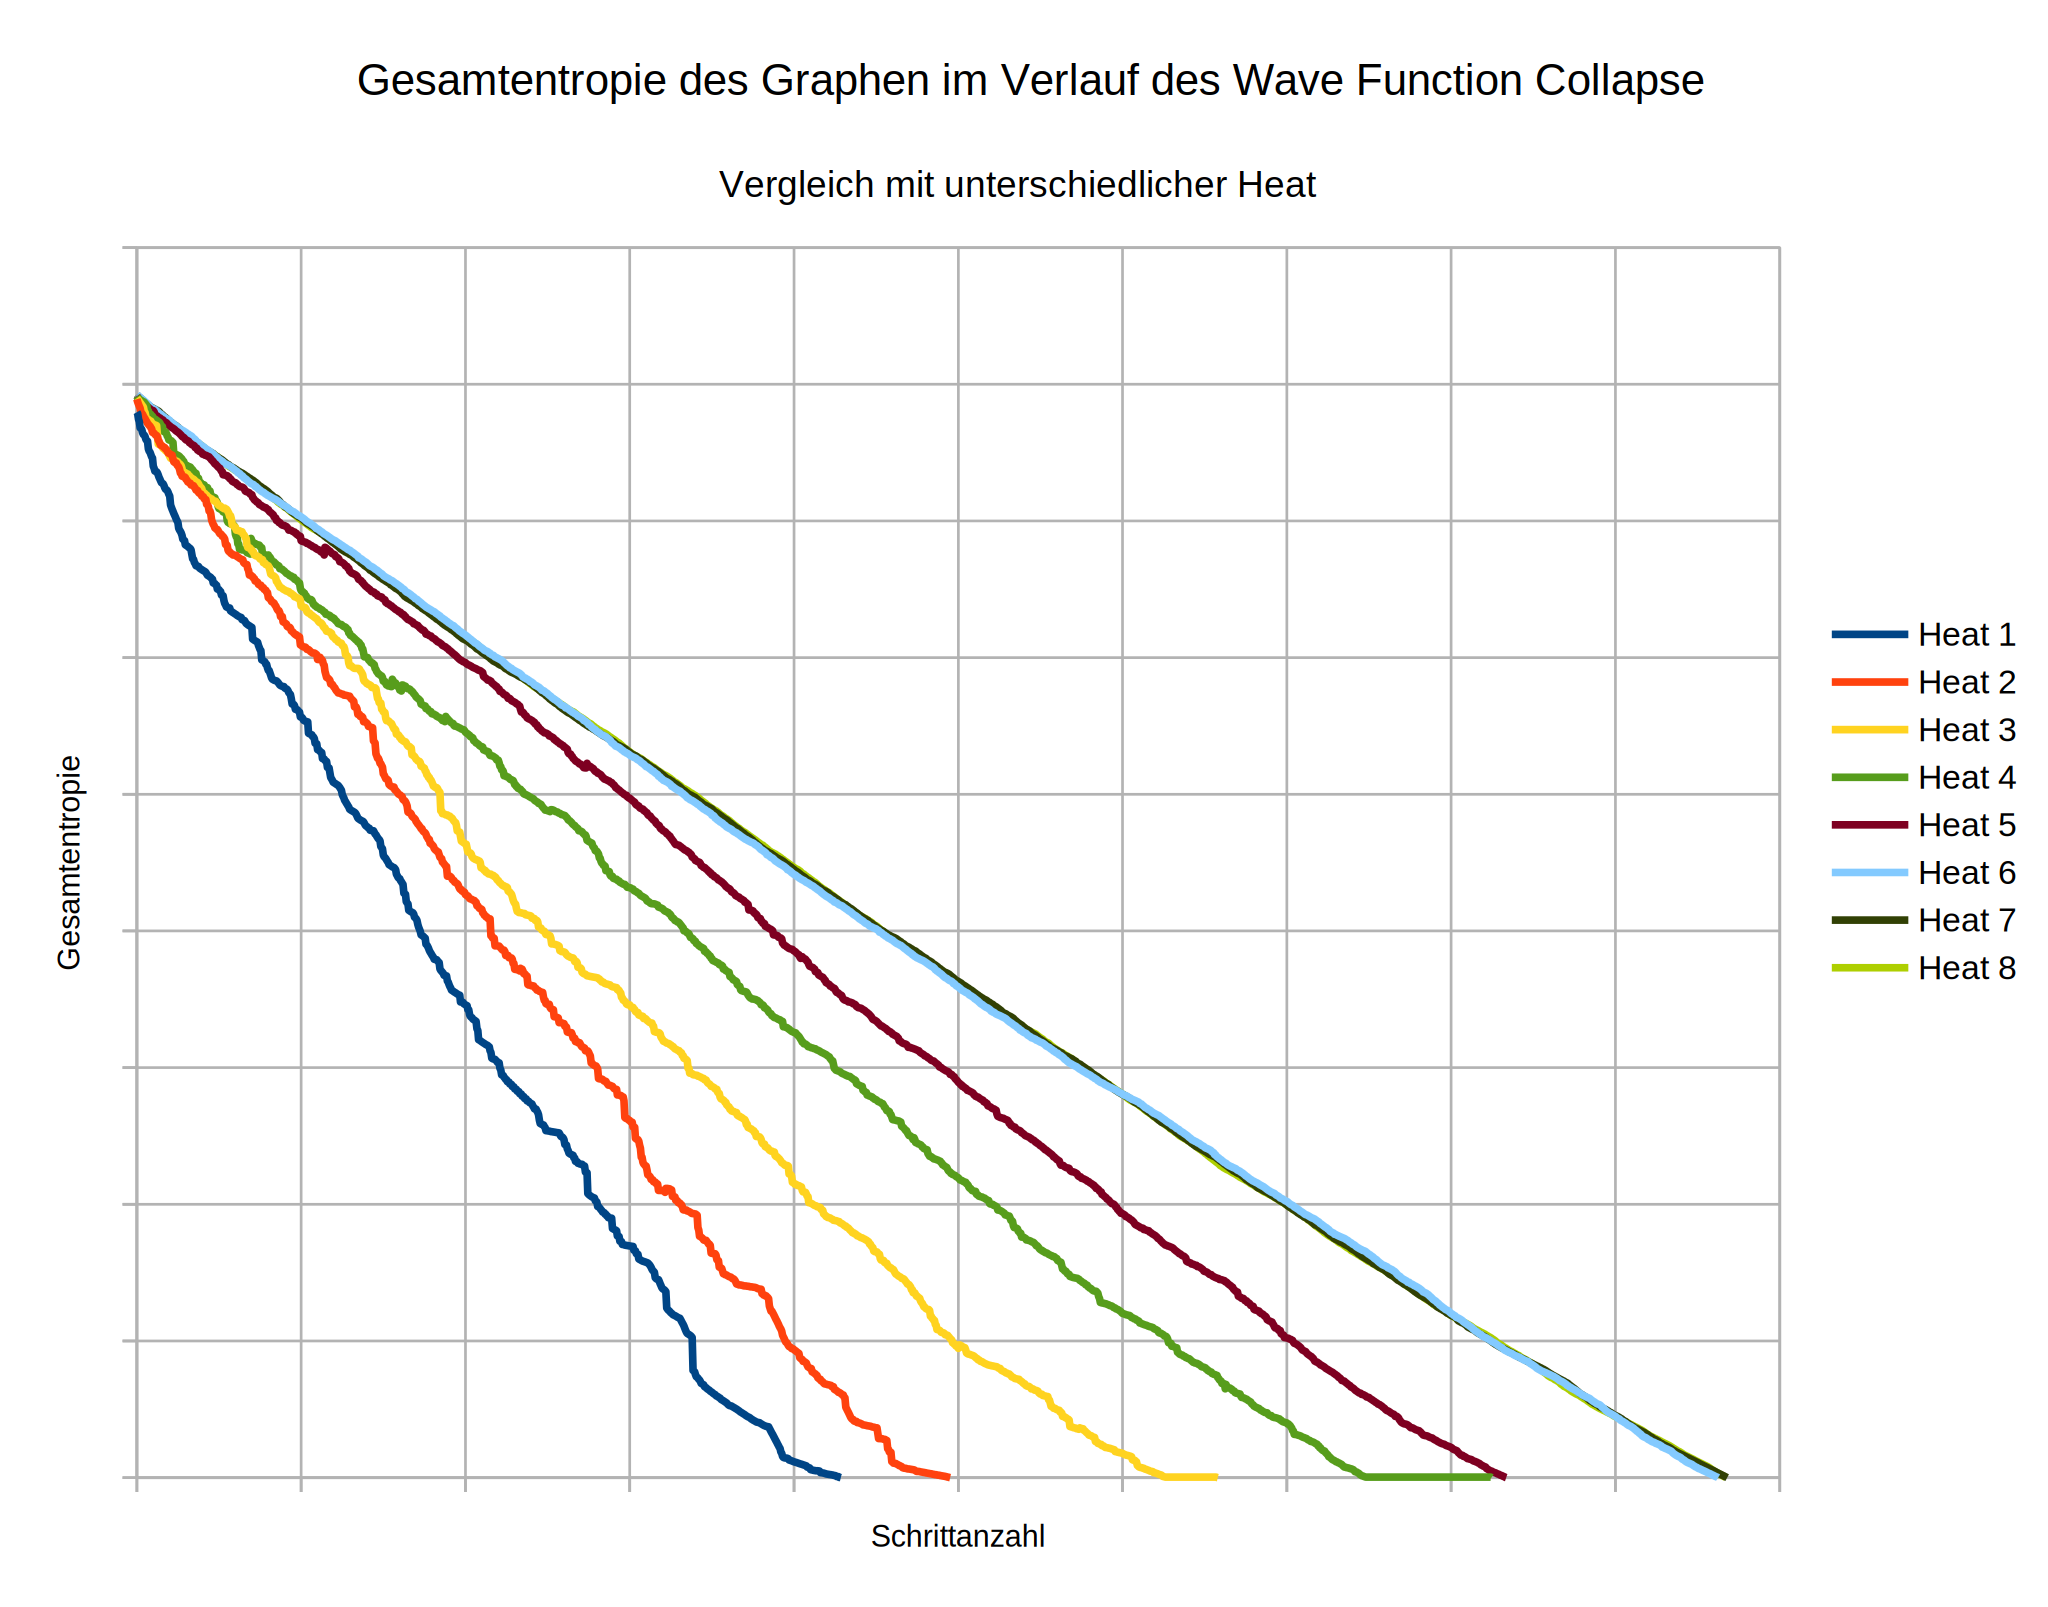
\includegraphics[width=\linewidth]{data/aliasing/1.png}  \caption{} \end{subfigure}
    
    \caption{
        Kurven und organische Formen lassen nicht exakt auf einem Gitter darstellen, es kommt zu Aliasing.
    }
    \label{fig:aliasing}
\end{figure}